\documentclass[12pt]{article}

% packages :
\usepackage[utf8x]{inputenc}
\usepackage[T1]{fontenc}
%\usepackage[francais]{babel}
%
\usepackage{graphicx} % images
\usepackage{float}
\usepackage{placeins}
\usepackage{multirow}
\usepackage{wrapfig}
\usepackage{array}

% to draw circuits
\usepackage{siunitx}
\usepackage{tikz}
\usetikzlibrary{calc}
\usetikzlibrary{decorations.pathmorphing,patterns,positioning}

\usepackage[top=2cm, bottom=2cm, left=2.5cm, right=2.5cm]{geometry}


% maths :
\usepackage{amsthm}
\usepackage{amsmath}
\usepackage{amssymb}
\usepackage{mathrsfs}

\usepackage{braket}

\begin{document}

\begin{center}
	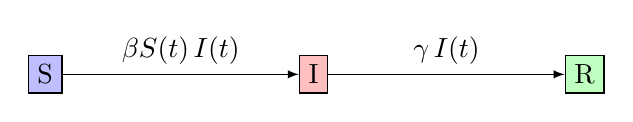
\begin{tikzpicture}
		\node[draw,fill=blue!25] (S) {S};
		\node[draw,fill=red!25,right=3cm of S] (I) {I};
		\node[draw,fill=green!25,right=3cm of I] (R) {R};
		\draw[-latex] (S.east) -- (I.west) node[midway,above]{$\beta S(t)\,I(t)$};
		\draw[-latex] (I.east) -- (R.west) node[midway,above]{$\gamma\,I(t)$};
	\end{tikzpicture}
\end{center}

\begin{center}
	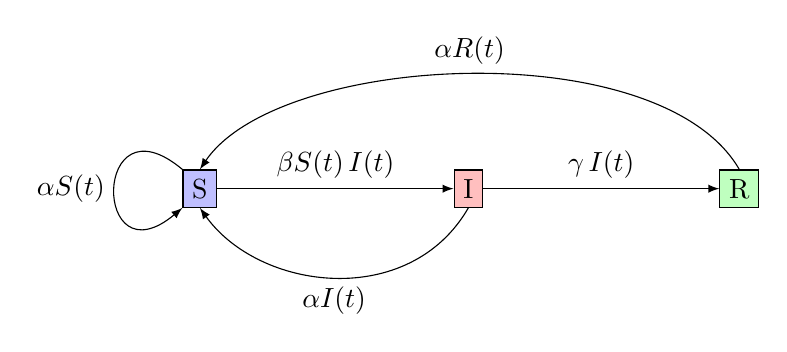
\begin{tikzpicture}
		\node[draw,fill=blue!25] (S) {S};
		\node[draw,fill=red!25,right=3cm of S] (I) {I};
		\node[draw,fill=green!25,right=3cm of I] (R) {R};
		\draw[-latex] (S.east) -- (I.west) node[midway,above]{$\beta S(t)\,I(t)$};
		\draw[-latex] (I.east) -- (R.west) node[midway,above]{$\gamma\,I(t)$};
		\draw[-latex] (I.south) .. controls +(240:1.5) and (-60:1.5) .. (S.south) node[midway,below]{$\alpha I(t)$};
		\draw[-latex] (R.north) .. controls +(120:2) and (60:2) .. (S.north) node[midway,above]{$\alpha R(t)$};
		\draw[-latex] (S.north west) .. controls +(140:1.5) and +(220:1.5) .. (S.south west) node[midway,left]{$\alpha S(t)$};
	\end{tikzpicture}
\end{center}

\end{document}
